\section{User Interface Design}

    \subsection{Desktop Interface}

    \href{https://www.figma.com/design/ZMtwuBt3jj4DOkPbbY6ElO/dota-stats?node-id=0-1&t=I0Mi3I4WJnfS4DOc-1}{\textbf{Figma project link}}.

    \vspace{1em}
    Starting page has simple layout.
    It presents 3 main pages of our website:
    \begin{itemize}
        \item Player's profile: check player's statistics.
        \item Heroes meta: check overall statistics of all heroes at the moment.
        \item Hero's stats: check analytical data for one selected hero.
    \end{itemize}


    \begin{figure}[ht]
        \centering
        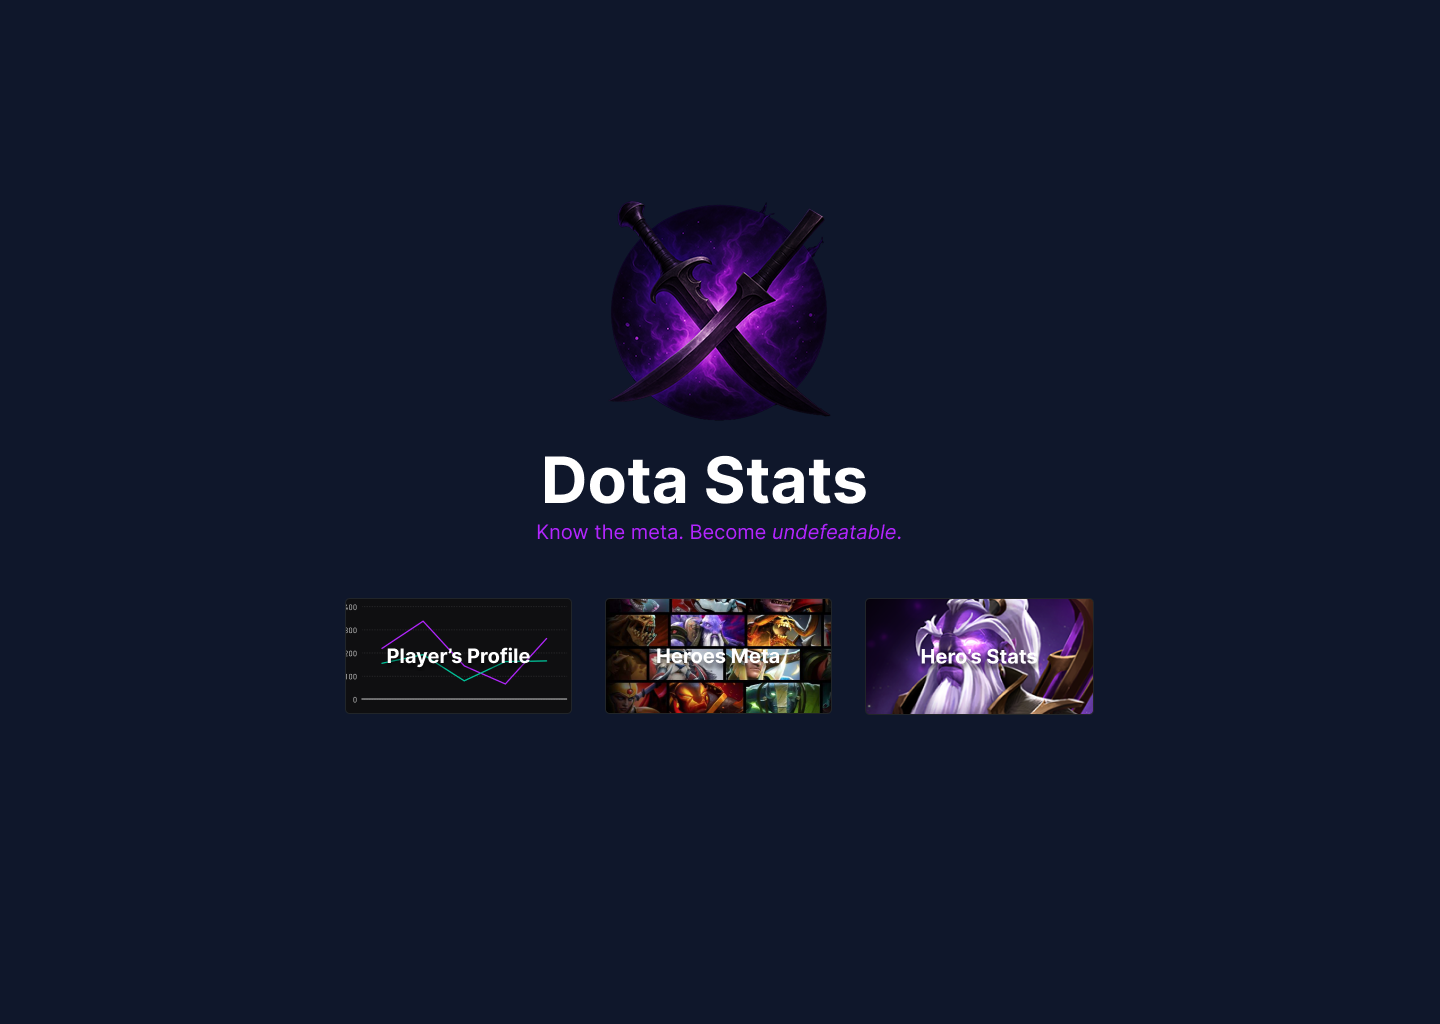
\includegraphics[width=0.8\textwidth]{images/Start}
        \caption{Start page}
    \end{figure}

    When user enters Player's profile page, they see a distribution of all playerbase in ranks (fig.~\ref{fig:rankDistr}).

    \begin{figure}[ht]
        \centering
        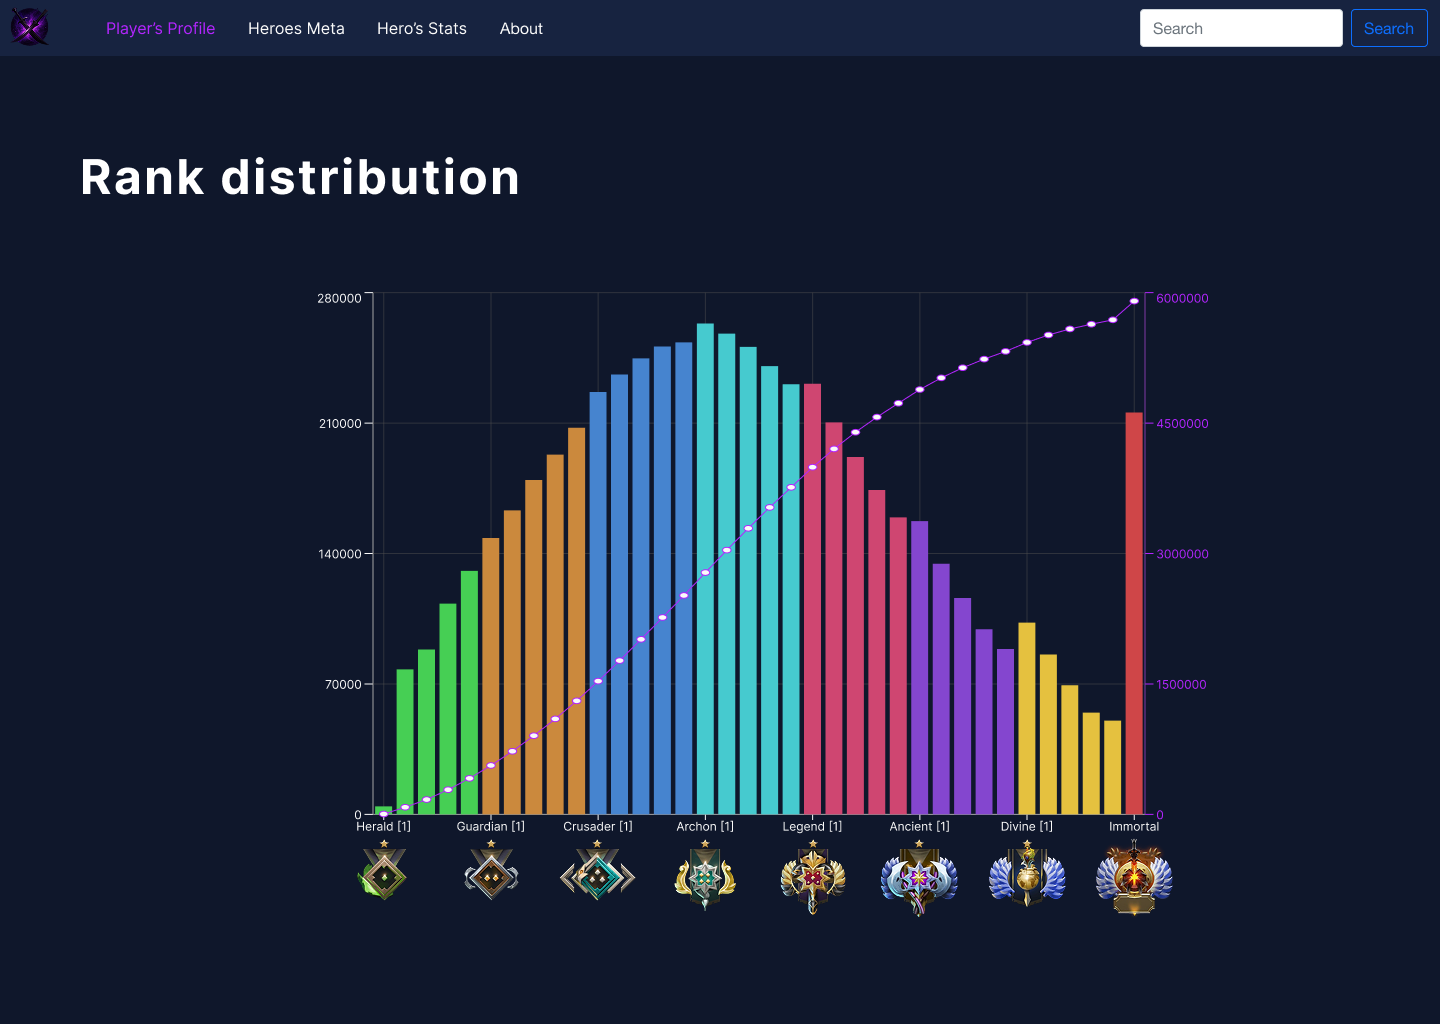
\includegraphics[width=0.8\textwidth]{images/PlayerProfileStartPage}
        \caption{Player's profile page before search}
        \label{fig:rankDistr}
    \end{figure}

    \begin{figure}[ht]
        \centering
        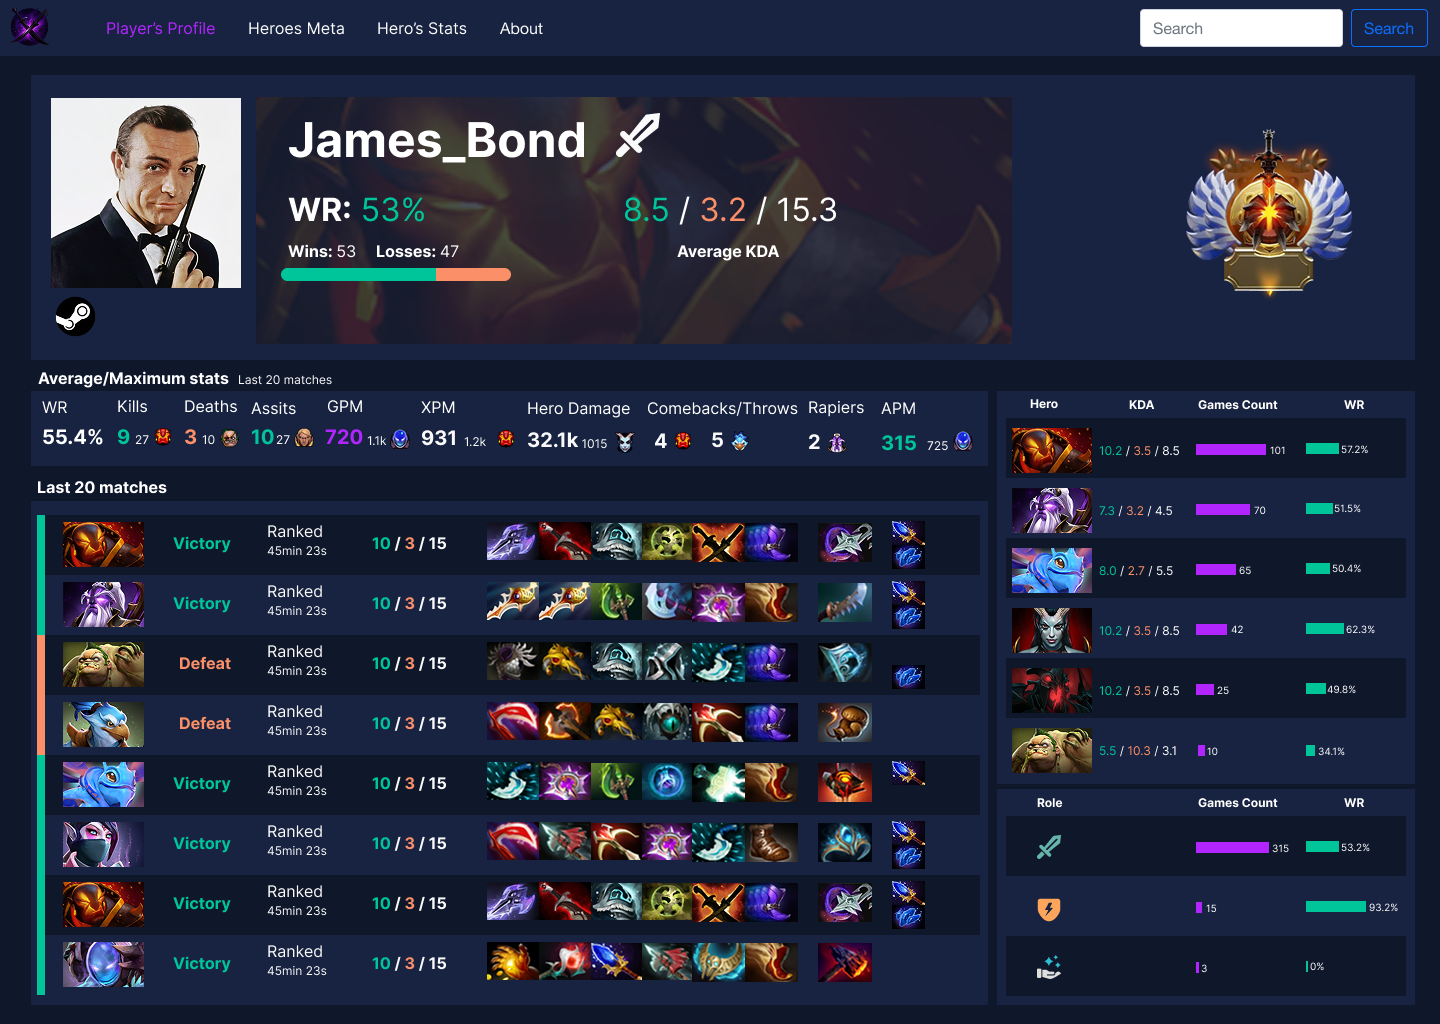
\includegraphics[width=0.8\textwidth]{images/PlayerProfile}
        \caption{Player's profile page after search (Successful search)}
    \end{figure}

    \begin{figure}[ht]
        \centering
        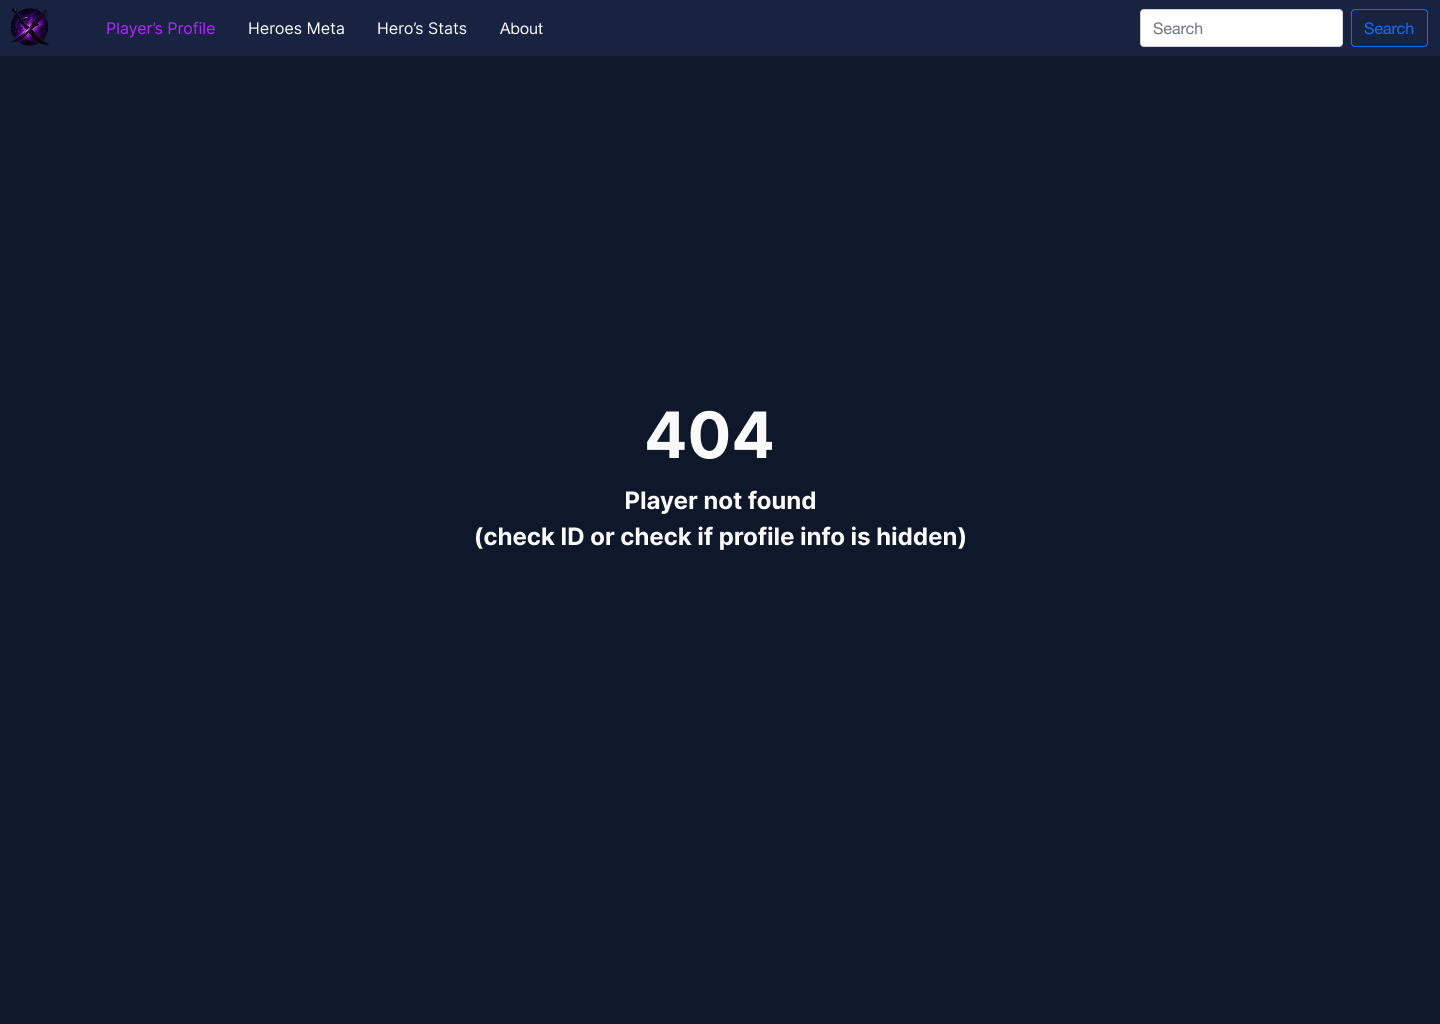
\includegraphics[width=0.8\textwidth]{images/PlayerNotFound}
        \caption{Player's profile page after search (Unsuccessful search)}
    \end{figure}

    \begin{figure}[ht]
        \centering
        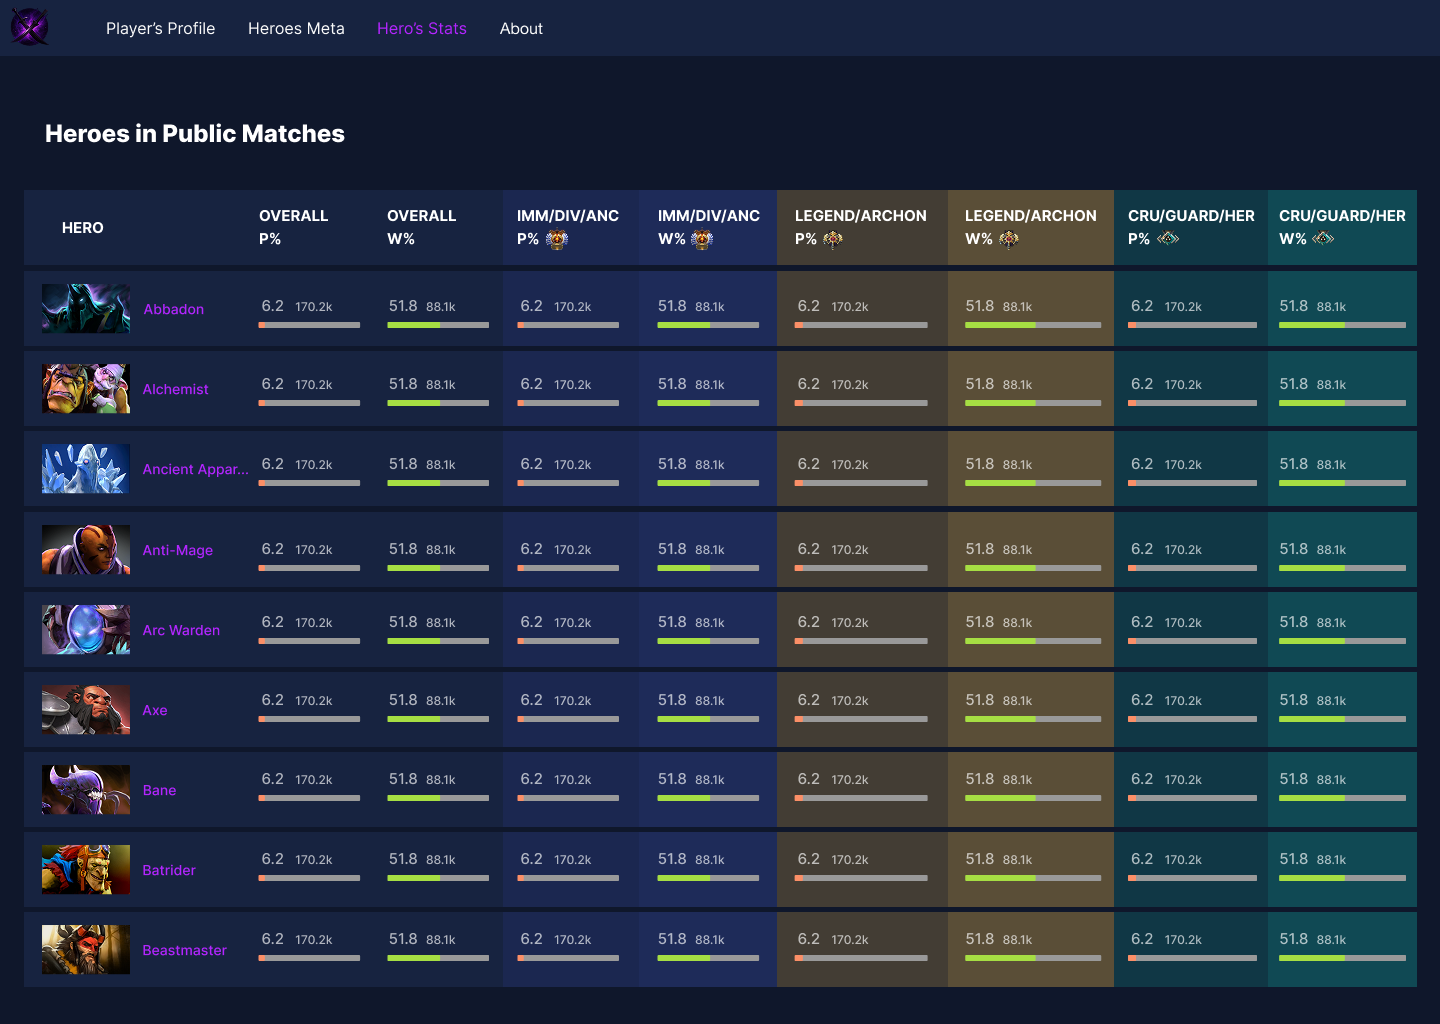
\includegraphics[width=0.8\textwidth]{images/HeroStats}
        \caption{Heroes statistics (Win, pick and ban rates in different ranks grouped)}
    \end{figure}

    \begin{figure}[ht]
        \centering
        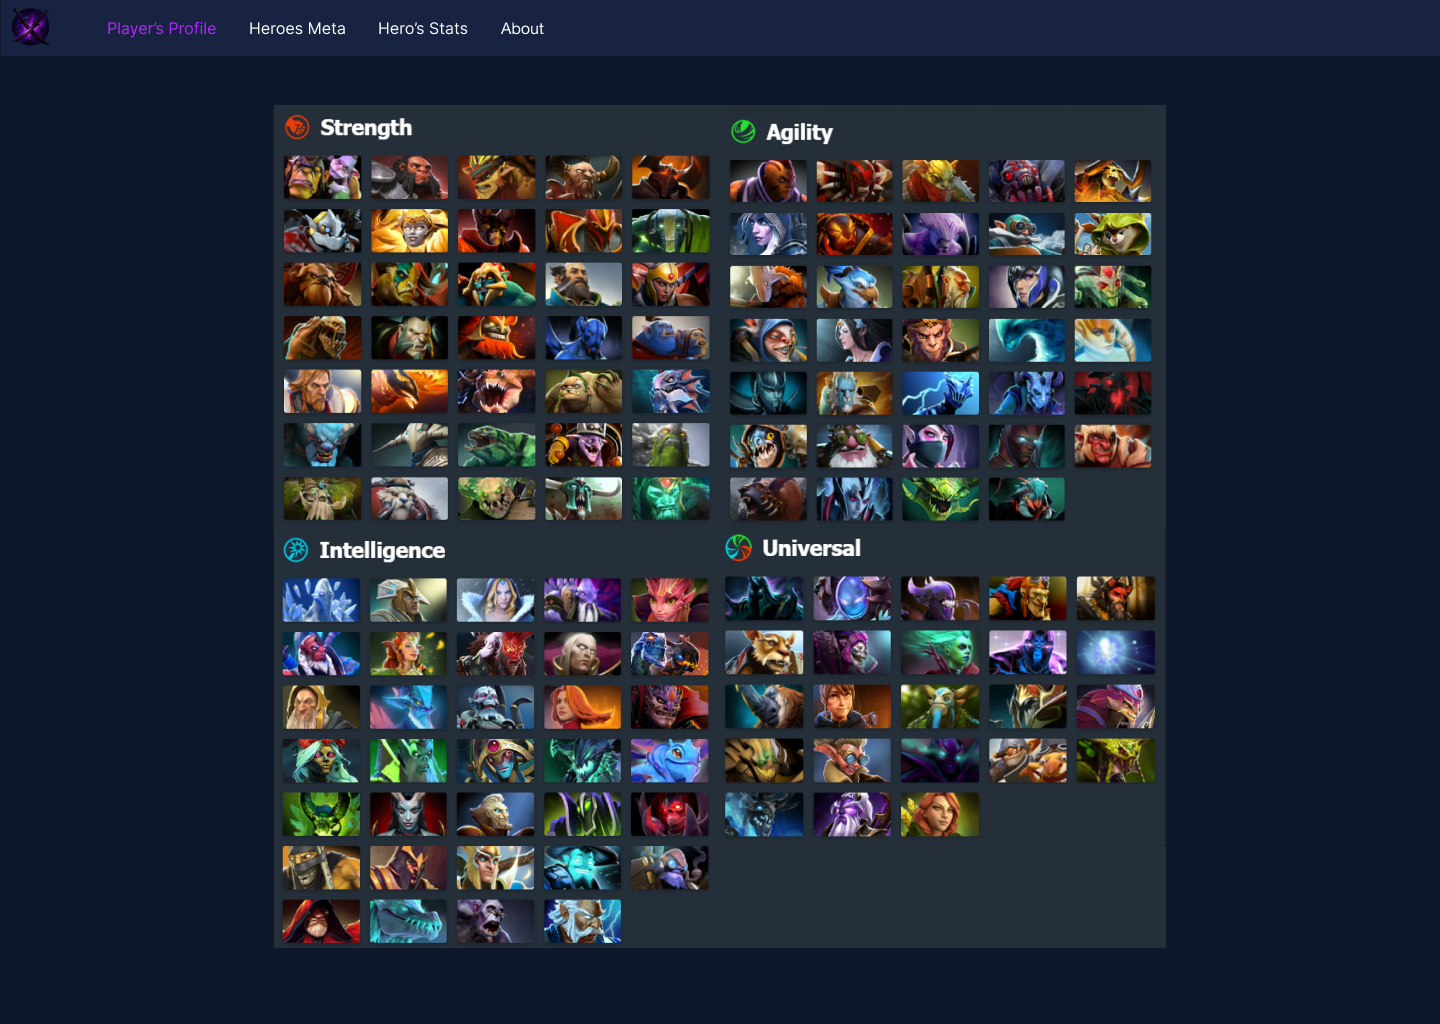
\includegraphics[width=0.9\textwidth]{images/HeroMatrix}
        \caption{Heroes Matrix (here user selects one hero to have detailed view)}
    \end{figure}

    \begin{figure}[ht]
        \centering
        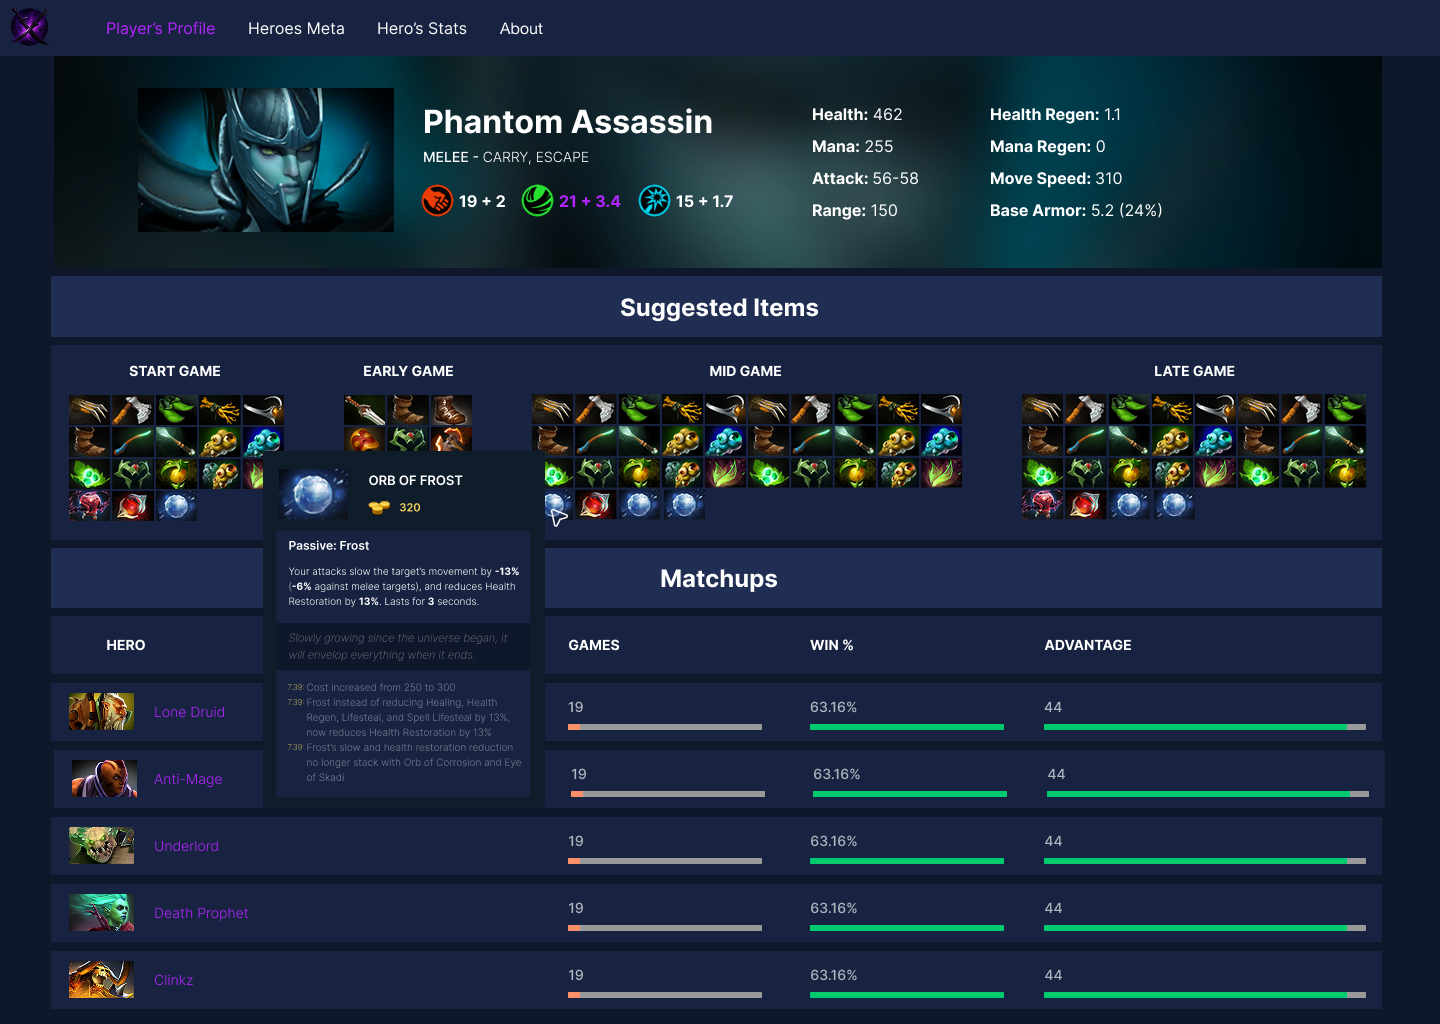
\includegraphics[width=0.9\textwidth]{images/SelectedHero}
        \caption{Statistics for one selected hero. Tooltip shows detailed item information.}
    \end{figure}

    \clearpage

    \subsection{Mobile}

    Our users will use the website in desktop mode in the majority of time (due to the fact that \("\)Dota \(2"\)\('\)s only platform is desktop).

    \vspace{1em}
    However, below are shown the 2 screens with dedicated mobile layout.

    \vspace{1em}
    Other screens either have big tables and, therefore, require horizontal scrolling, hence desktop and mobile versions of the layout are the same in this case
    or have small amount of details and therefore there are no major changes in layout.

    \begin{figure}[ht]
        \centering
        \begin{minipage}[t]{0.48\textwidth}
            \centering
            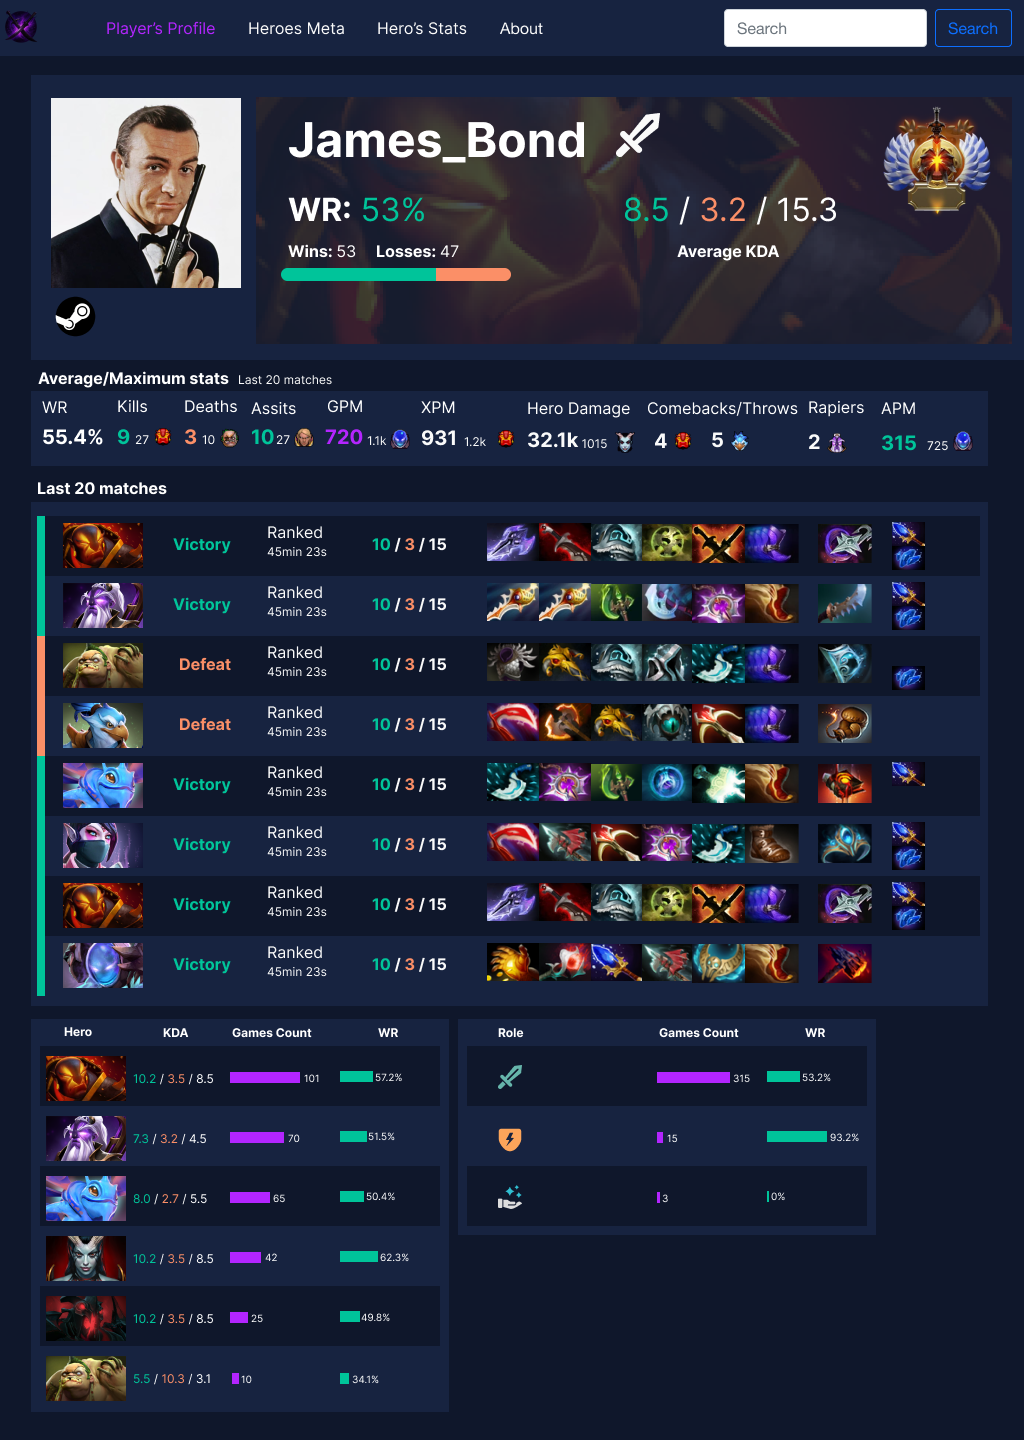
\includegraphics[width=\textwidth]{images/PlayerProfile_m}
            \caption{Player's profile (mobile)}
        \end{minipage}
        \hfill
        \begin{minipage}[t]{0.48\textwidth}
            \centering
            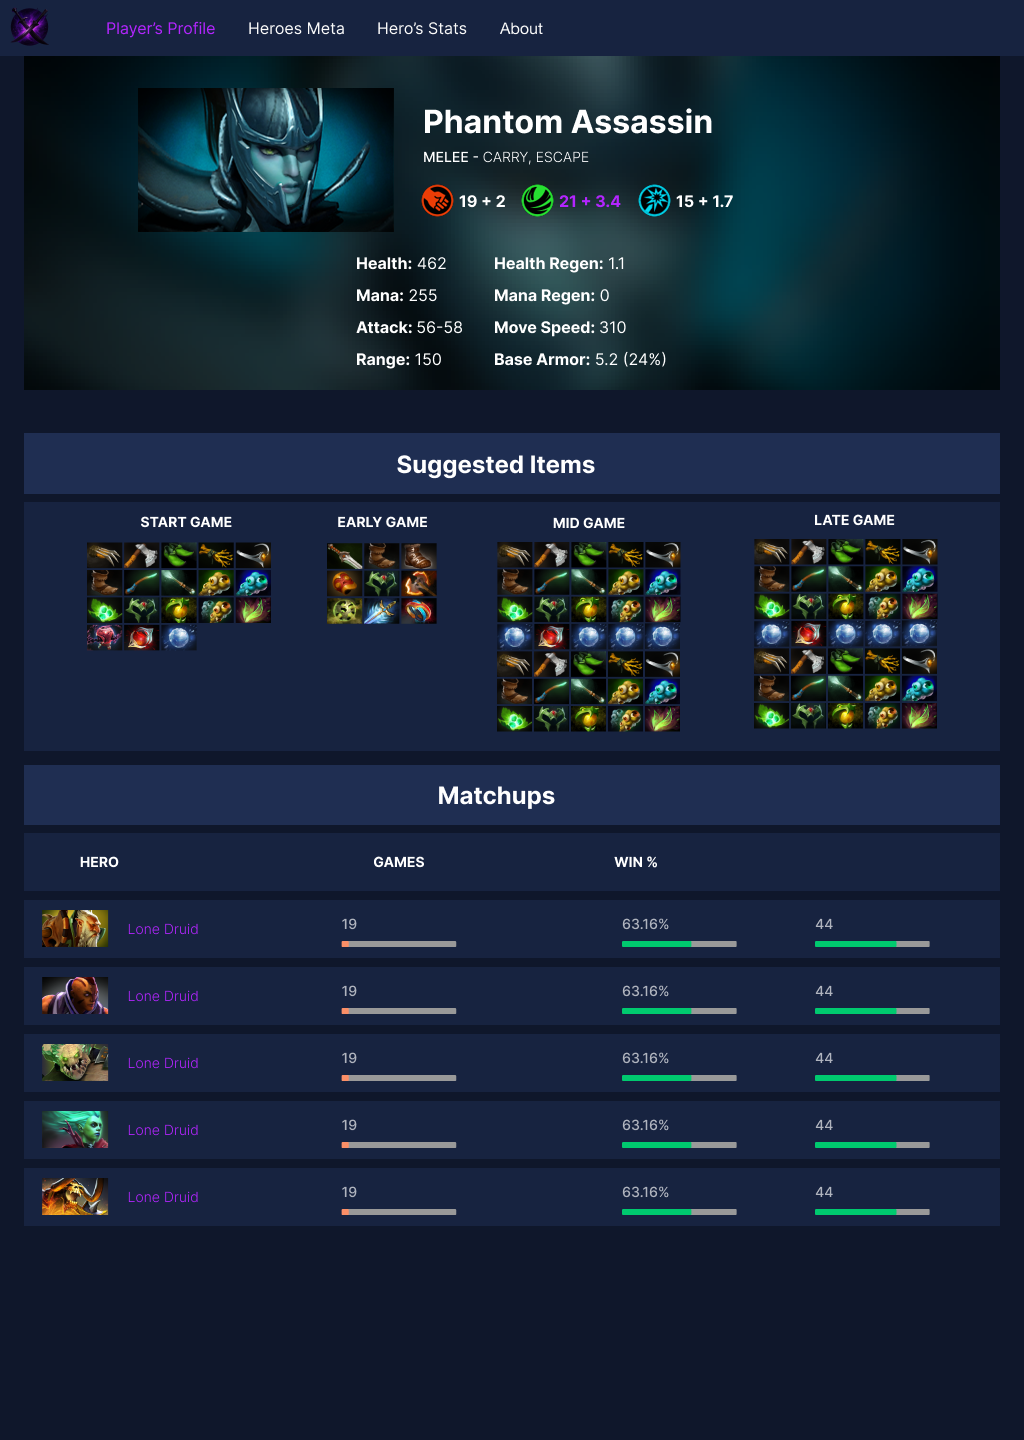
\includegraphics[width=\textwidth]{images/SelectedHero_m}
            \caption{Selected hero (mobile)}
        \end{minipage}
    \end{figure}



    \subsection{References}
        For designing our website we analyzed existing websites of same category.
        List of references (links to particular pages):
        \begin{itemize}
            \item \href{https://www.opendota.com/heroes/public}{OpenDota}
            \item \href{https://www.dotabuff.com/esports/players/321580662-yatoro}{DotaBuff}
            \item \href{https://www.leagueofgraphs.com/summoner/ru/L9+Capybara-ff15}{LeagueOfGraphs}
            \item \href{https://lolalytics.com/de/lol/katarina/build/}{Lolalytics}
            \item \href{https://stratz.com/players/ranks}{Stratz}
        \end{itemize}

        Screenshots of most used references:

    \begin{figure}[ht]
        \centering
        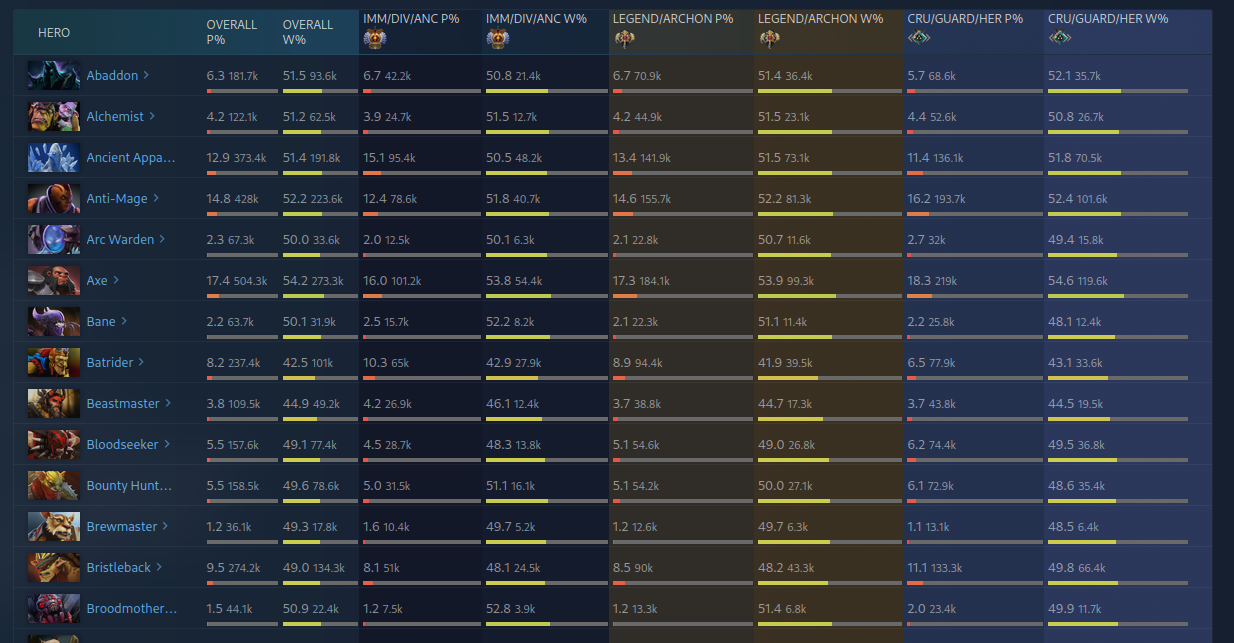
\includegraphics[width=1\textwidth]{images/references/OpenDota1}
        \caption{OpenDota. Win, pick and ban rates of heroes.}
    \end{figure}

    \begin{figure}[ht]
        \centering
        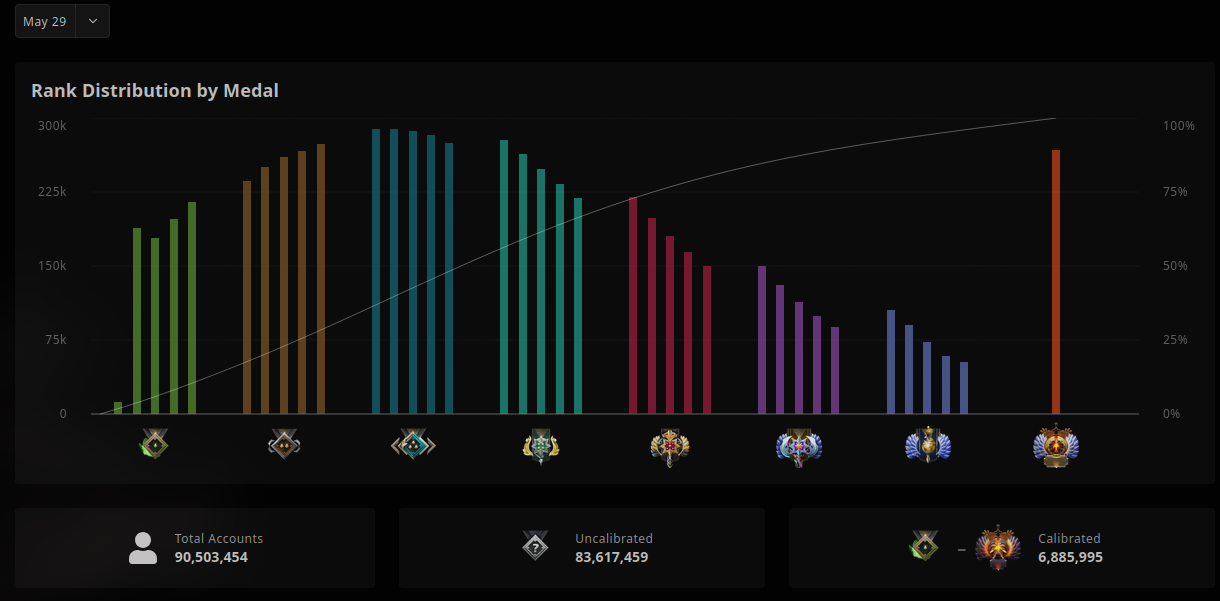
\includegraphics[width=1\textwidth]{images/references/Stratz}
        \caption{Stratz. Players rank distribution}
    \end{figure}

    \begin{figure}[ht]
        \centering
        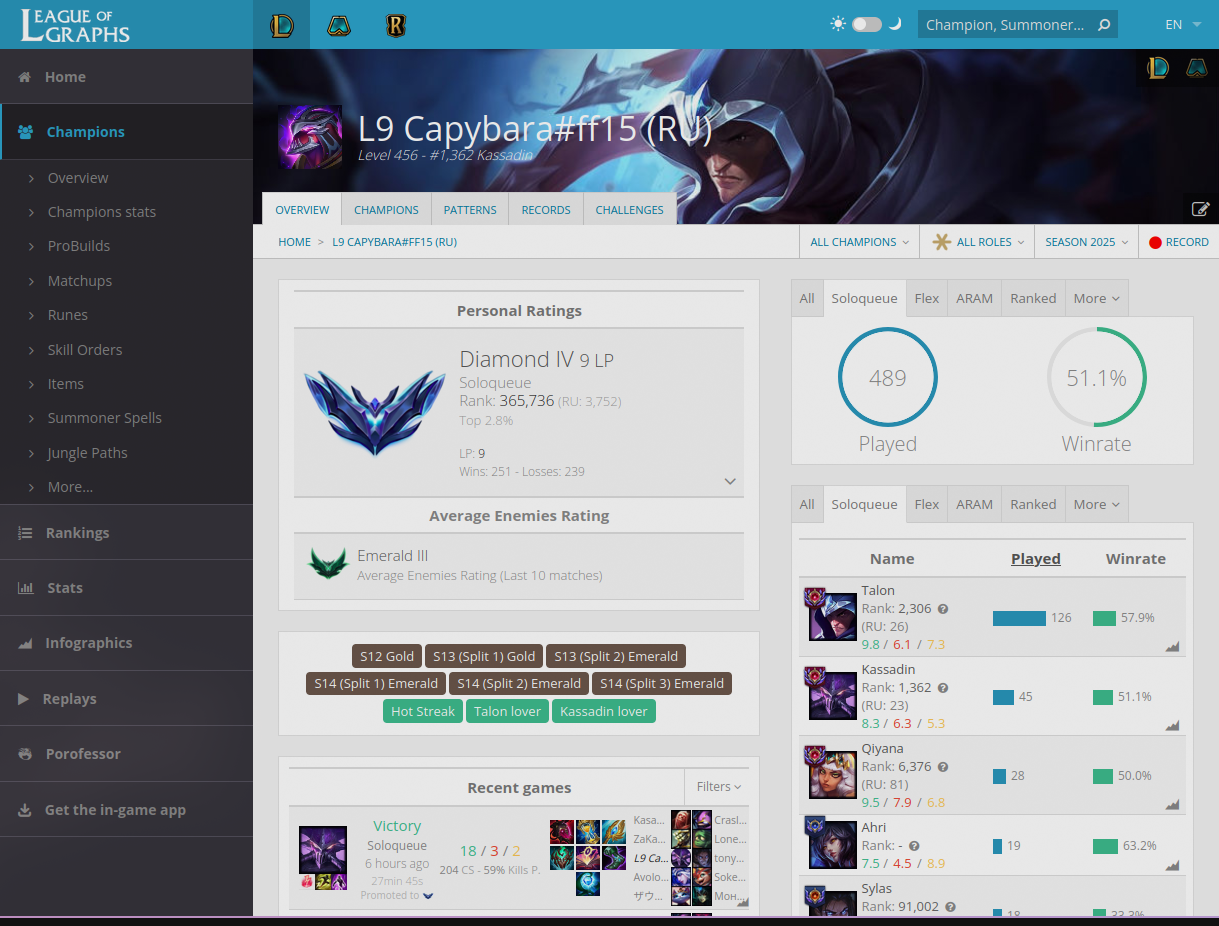
\includegraphics[width=1\textwidth]{images/references/LoG}
        \caption{LeagueOfGraph. Layout and most played heroes and roles.}
    \end{figure}

    \begin{figure}[ht]
        \centering
        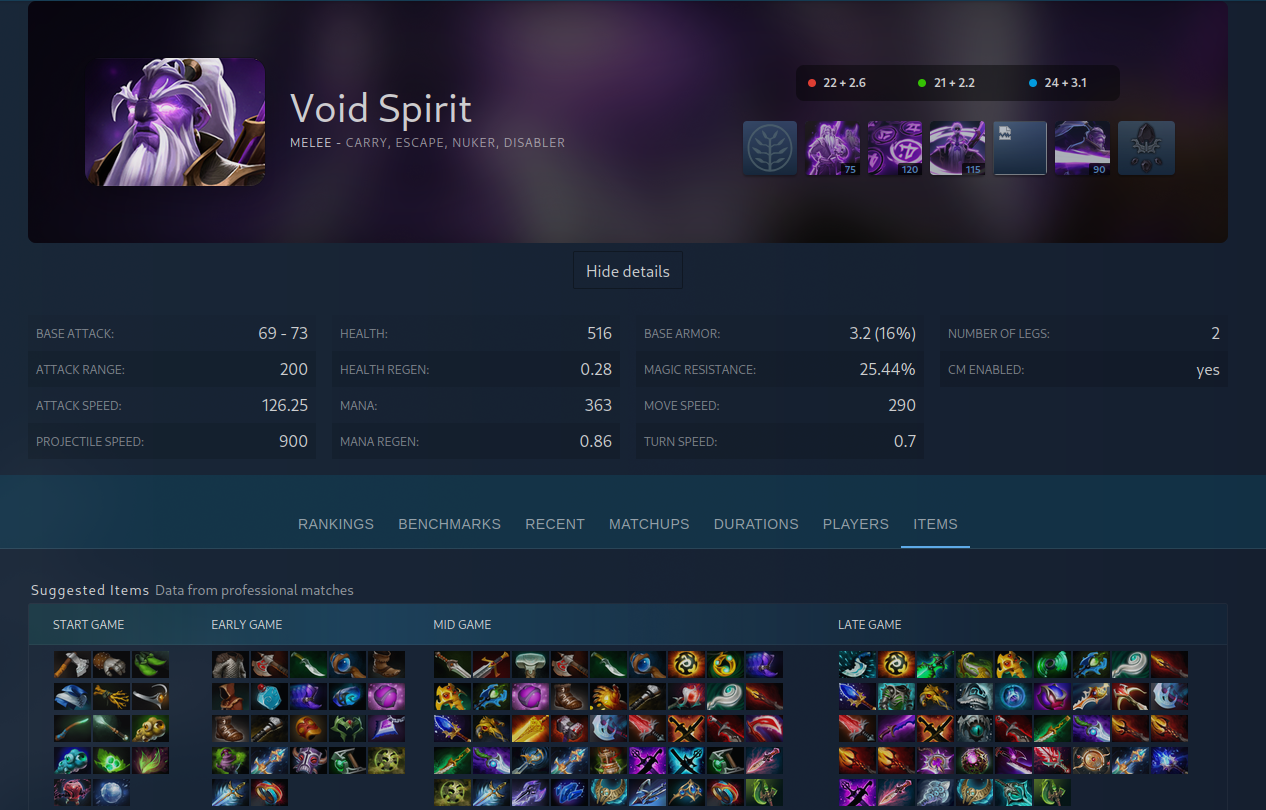
\includegraphics[width=1\textwidth]{images/references/OpenDota2}
        \caption{OpenDota. Data for selected hero.}
    \end{figure}

    \begin{figure}[ht]
        \centering
        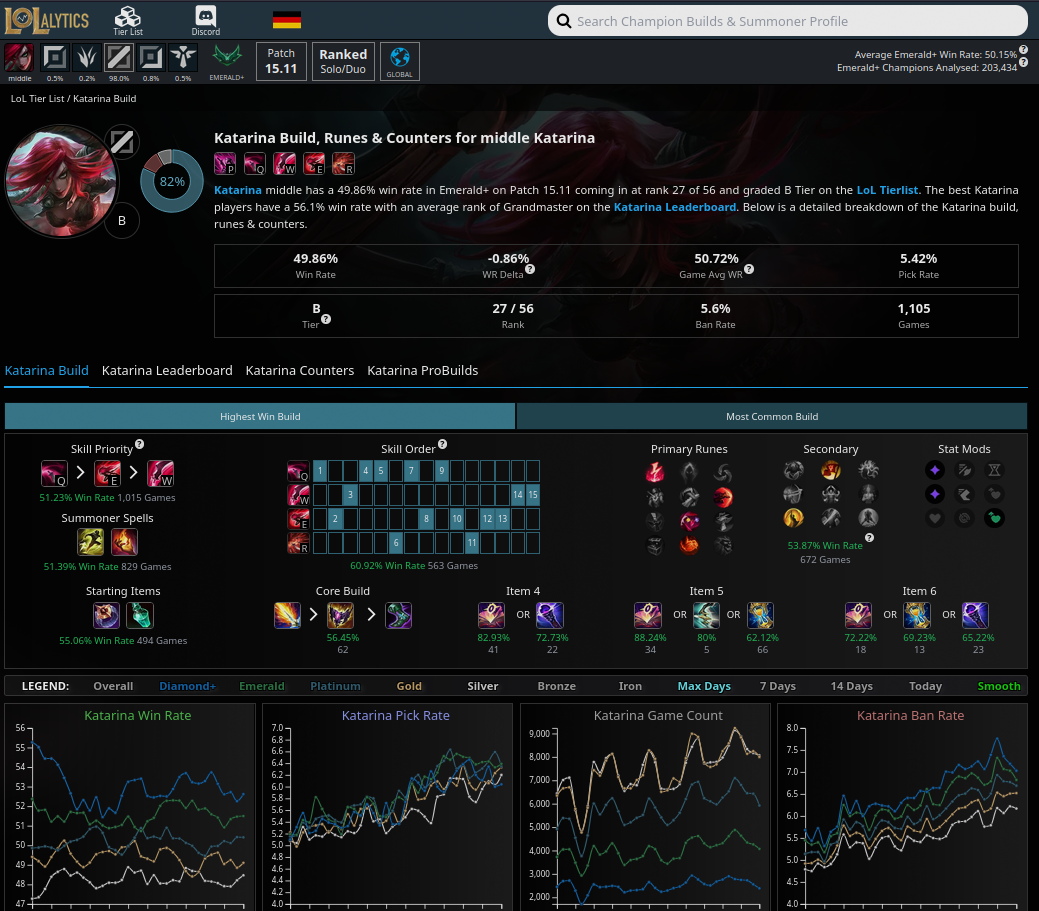
\includegraphics[width=0.85\textwidth]{images/references/Lolalytics}
        \caption{Lolalytics. Parts of layout, general insperation.}
    \end{figure}

    \begin{figure}[ht]
        \centering
        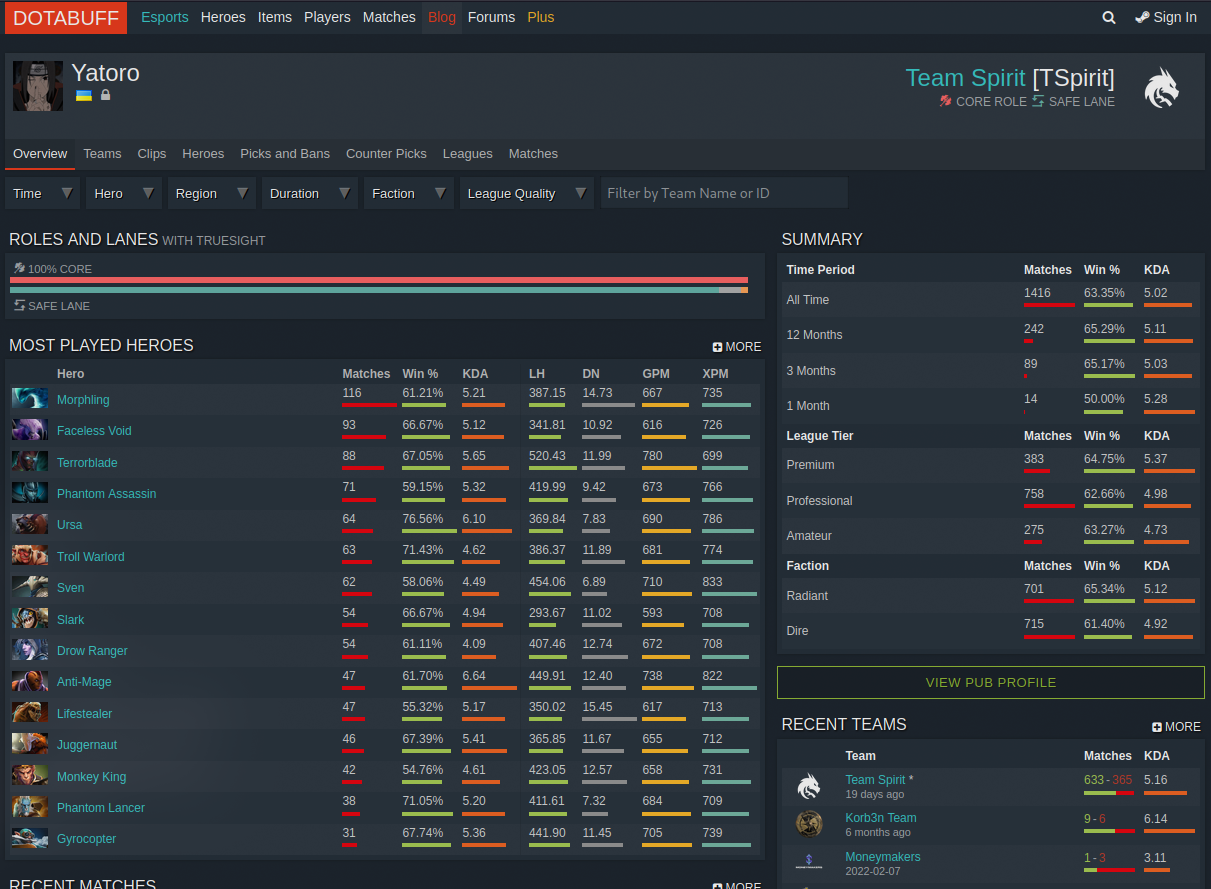
\includegraphics[width=0.85\textwidth]{images/references/DotaBuff}
        \caption{DotaBuff. Parts of layout, general insperation.}
    \end{figure}


    \clearpage

